\begin{figure}[tbh]
\centering
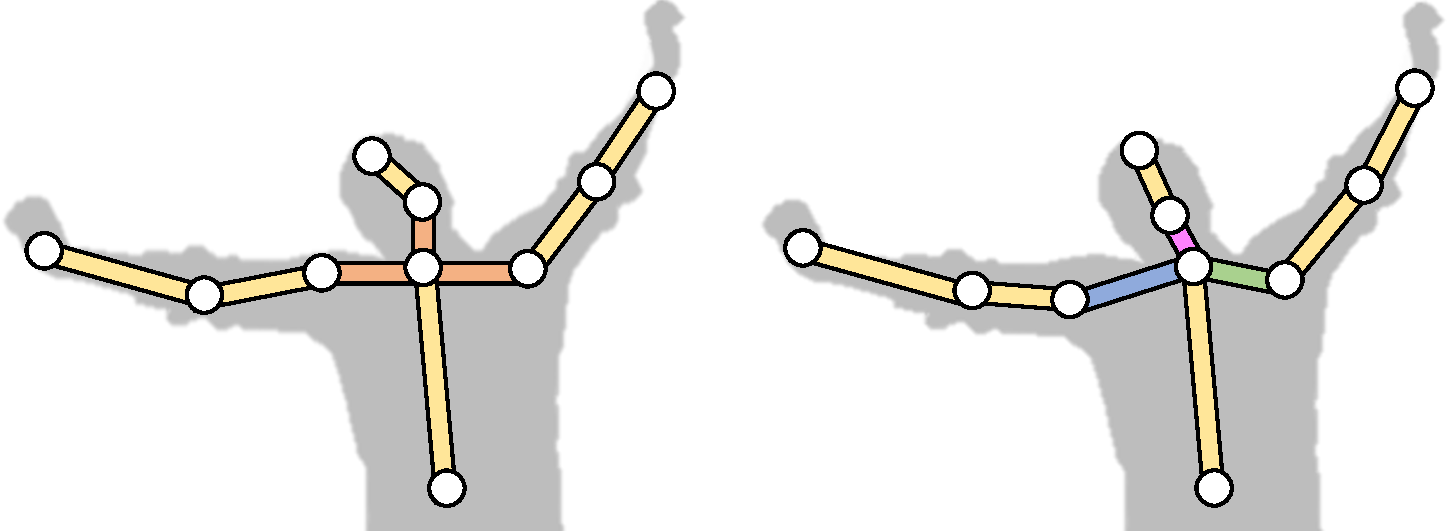
\includegraphics[width=\linewidth]{./images/Skeleton_Difference_Shoulders.pdf}
\setlength{\abovecaptionskip}{-5pt plus 3pt minus 2pt}
\setlength{\belowcaptionskip}{-3pt plus 3pt minus 2pt}
\caption{Skeletal connectivity changes, demonstrated on the neck joint. Left: original connectivity, where shoulders and head are rigidly connected, yielding poor reconstruction. Right: new connectivity, with extra degrees of freedom. }
\label{fig:skeletal_change}
\end{figure}